%==========================================================
% CHAPTER 6: Stochastika
%==========================================================
\chapter{Stochastika (Duomenys ir tikimybės)}

\section{Kombinatorika}

\textbf{Kombinatorika} -- tai matematikos šaka, nagrinėjanti baigtinių aibių elementų rinkinių sudarymo ir skaičiavimo metodus. Pagrindiniai klausimai: \emph{kiek skirtingų rinkinių galima sudaryti iš duotų elementų?}, \emph{ar svarbi elementų tvarka?}, \emph{ar elementai gali kartotis?} Kombinatorikos metodai plačiai taikomi tikimybių teorijoje, informatikoje ir optimizavimo uždaviniuose.

\begin{definition}[Faktorialas]
Natūraliojo skaičiaus $n$ \textbf{faktorialas} (žymimas $n!$) yra visų natūraliųjų skaičių nuo $1$ iki $n$ sandauga:
\[
n! = 1 \cdot 2 \cdot 3 \cdots (n-1) \cdot n = \prod_{i=1}^{n} i.
\]
Sutartinai laikoma, kad $0! = 1$.
\end{definition}

\begin{example}
\[
1! = 1, \quad 2! = 2, \quad 3! = 6, \quad 4! = 24, \quad 5! = 120, \quad 6! = 720, \quad 10! = 3\,628\,800.
\]
\end{example}

\begin{remark}
Naudinga pastaba: $n! = n \cdot (n-1)!$, todėl faktorialus galima skaičiuoti rekursiškai.
\end{remark}

Prieš nagrinėjant pagrindinius kombinatorinius objektus, suformuluosime dvi pagrindines taisykles, kuriomis grindžiama visa kombinatorika.

\begin{theorem}[Daugybos taisyklė]
Jei veiksmų seka susideda iš $m$ nepriklausomų žingsnių, kuriuos galima atlikti atitinkamai $n_1, n_2, \ldots, n_m$ būdais, tai visa seka gali būti įvykdyta
\[
n_1 \cdot n_2 \cdots n_m
\]
būdų.
\end{theorem}

\begin{theorem}[Sudėties taisyklė]
Jei kokį nors objektą galima pasirinkti vienu iš $A_1, A_2, \ldots, A_k$ nesuderinimų (nesikertančių) būdų, kurių kiekvienas duoda atitinkamai $n_1, n_2, \ldots, n_k$ variantų, tai iš viso yra
\[
n_1 + n_2 + \cdots + n_k
\]
galimų variantų.
\end{theorem}

\begin{example}
Penkiaženklio kodo pirmasis simbolis -- raidė (iš 26 raidžių), o kiti keturi -- skaitmenys (nuo 0 iki 9). Pagal daugybos taisyklę, galimų kodų skaičius:
\[
26 \cdot 10 \cdot 10 \cdot 10 \cdot 10 = 26 \cdot 10^4 = 260\,000.
\]
\end{example}

% -------------------------------------------------------
\subsection{Kėliniai}
% -------------------------------------------------------

\textbf{Kėliniai} -- tai visi galimi $n$ skirtingų elementų pertvarkymai, kai naudojami \emph{visi} elementai ir jų tvarka yra svarbi.

\begin{definition}[Kėliniai]
$n$ skirtingų elementų \textbf{kėliniais} vadinami visi galimi šių elementų išdėstymai skirtinga tvarka. Kėlinių skaičius žymimas $P_n$ arba $n!$:
\[
P_n = n! = 1 \cdot 2 \cdot 3 \cdots n.
\]
\end{definition}

\begin{proof}[Pagrindimas]
Pirmąją vietą galima užimti $n$ būdų, antrąją -- $n-1$ likusių būdų, ir t.\,t., kol paskutinę vietą galima užimti tik $1$ būdu. Pagal daugybos taisyklę:
\[
P_n = n \cdot (n-1) \cdot (n-2) \cdots 2 \cdot 1 = n!.
\]
\end{proof}

\begin{example}
Keliais būdais galima sudėti $5$ skirtingas knygas į lentynos eilę?

Kadangi naudojamos visos $5$ knygos ir tvarka svarbi:
\[
P_5 = 5! = 120.
\]
\end{example}

\begin{example}
Kiek skirtingų eilių galima susodinti $8$ mokinius ant suoliuko?
\[
P_8 = 8! = 40\,320.
\]
\end{example}

\subsubsection*{Gretiniai}

Kėliniai yra specialus atvejis platesnės sąvokos -- \textbf{gretinių}, kai iš $n$ elementų imame tik dalį $k \leq n$ ir tvarka svarbi.

\begin{definition}[Gretiniai]
$n$ skirtingų elementų \textbf{gretiniais po $k$} vadinami visi galimi $k$ elementų rinkiniai, sudaryti iš šių $n$ elementų, kai elementų tvarka svarbi. Gretinių skaičius žymimas $A_n^k$:
\[
A_n^k = \frac{n!}{(n-k)!} = n \cdot (n-1) \cdots (n-k+1).
\]
\end{definition}

\begin{remark}
Kėliniai yra specialus gretinių atvejis, kai $k = n$:
\[
A_n^n = \frac{n!}{(n-n)!} = \frac{n!}{0!} = n! = P_n.
\]
\end{remark}

\begin{example}
Iš $8$ bėgikų dalyvių paskiriamos I, II ir III vietos. Kiek yra galimų rezultatų?

Tvarka svarbi (skiriasi I, II ir III vieta), naudojami $3$ iš $8$ elementų:
\[
A_8^3 = \frac{8!}{(8-3)!} = \frac{8!}{5!} = 8 \cdot 7 \cdot 6 = 336.
\]
\end{example}

\begin{example}
Kiek skirtingų $4$ raidžių žodžių (nebūtinai prasmingų) galima sudaryti iš lotyniško alfabeto 26 raidžių, jei raidės nesikartoja?
\[
A_{26}^{4} = 26 \cdot 25 \cdot 24 \cdot 23 = 358\,800.
\]
\end{example}

\subsubsection*{Kėliniai su pasikartojimais}

\begin{definition}[Kėliniai su pasikartojimais]
Tarkime, turime $n$ elementų, kurių $n_1$ yra vienodo tipo, $n_2$ -- kito tipo ir t.\,t., kur $n_1 + n_2 + \cdots + n_r = n$. Tokiu atveju \textbf{kėlinių su pasikartojimais} skaičius yra:
\[
P(n_1, n_2, \ldots, n_r) = \frac{n!}{n_1!\, n_2! \cdots n_r!}.
\]
\end{definition}

\begin{example}
Kiek skirtingų žodžių galima sudaryti iš raidžių, sudarančių žodį \textsc{MATEMATIKA}?

Žodyje yra $10$ raidžių: M -- 2 kartus, A -- 3 kartus, T -- 2 kartus, E -- 1 kartą, I -- 1 kartą, K -- 1 kartą. Taigi:
\[
P(2, 3, 2, 1, 1, 1) = \frac{10!}{2!\cdot 3!\cdot 2!\cdot 1!\cdot 1!\cdot 1!} = \frac{3\,628\,800}{2 \cdot 6 \cdot 2 \cdot 1 \cdot 1 \cdot 1} = \frac{3\,628\,800}{24} = 151\,200.
\]
\end{example}

\begin{exercise}
Keliais būdais $9$ skirtingi žmonės gali išsirikiuoti eilėje?
\end{exercise}

\begin{exercise}
Iš $10$ komandos žaidėjų reikia išrinkti kapitoną, vicekaptioną ir atsarginį žaidėją. Kiek galima būdų tai padaryti?
\end{exercise}

\begin{exercise}
Kiek skirtingų anagramų turi žodis \textsc{LIETUVA}?
\end{exercise}

% -------------------------------------------------------
\subsection{Deriniai}
% -------------------------------------------------------

\textbf{Deriniai} -- tai $k$ elementų pogrupiai, sudaryti iš $n$ skirtingų elementų, kai tvarka \emph{nesvarbi}. Deriniai yra vienas dažniausiai naudojamų kombinatorikos objektų.

\begin{definition}[Deriniai]
$n$ skirtingų elementų \textbf{deriniais po $k$} vadinami visi galimi $k$ elementų poaibiai, sudaryti iš duotų $n$ elementų, kai jų tvarka nesvarbi. Derinių skaičius žymimas $C_n^k$ arba $\displaystyle\binom{n}{k}$:
\[
C_n^k = \binom{n}{k} = \frac{n!}{k!\,(n-k)!}, \quad 0 \leq k \leq n.
\]
\end{definition}

\begin{remark}
Ryšys tarp gretinių ir derinių:
\[
A_n^k = C_n^k \cdot k!,
\]
nes kiekvieną $k$ elementų derinį galima pertvarkyti $k!$ skirtingų kėlinių, taip gaunant atitinkamus gretinius.
\end{remark}

\begin{example}
Iš $10$ komandos narių reikia išrinkti $3$ atstovus delegacijai (postai nesiskiria). Kiek galimų pasirinkimų?

Tvarka neaktuali, todėl skaičiuojame derinius:
\[
C_{10}^{3} = \frac{10!}{3!\cdot 7!} = \frac{10 \cdot 9 \cdot 8}{3 \cdot 2 \cdot 1} = \frac{720}{6} = 120.
\]
\end{example}

\begin{example}
Lošimo kortos kaladėje yra $52$ kortos. Kiek galima išdalinti skirtingų $5$ kortų kombinacijų?
\[
C_{52}^{5} = \frac{52!}{5!\cdot 47!} = \frac{52 \cdot 51 \cdot 50 \cdot 49 \cdot 48}{120} = 2\,598\,960.
\]
\end{example}

\subsubsection*{Derinių savybės}

\begin{theorem}[Simetrijos savybė]
\[
C_n^k = C_n^{n-k}.
\]
Tai reiškia, kad pasirinkti $k$ elementų -- tas pats, kas \emph{neįtraukti} $n - k$ elementų.
\end{theorem}

\begin{corollary}
$C_n^0 = C_n^n = 1$ ir $C_n^1 = C_n^{n-1} = n$.
\end{corollary}

\begin{theorem}[Paskalio taisyklė]
\[
C_n^k = C_{n-1}^{k-1} + C_{n-1}^{k}, \quad 1 \leq k \leq n-1.
\]
Ši savybė reiškia, kad kiekvieną $k$ elementų derinį iš $n$ elementų galima arba \emph{įtraukti} fiksuotą $n$-ąjį elementą (ir papildyti $k-1$ iš likusių $n-1$) arba \emph{neįtraukti} jo (ir rinktis visus $k$ iš likusių $n-1$).
\end{theorem}

\subsubsection*{Paskalio trikampis}

Paskalio taisyklė leidžia sudaryti \textbf{Paskalio trikampį}, kuriame $n$-osios eilutės $k$-asis skaičius yra lygus $C_n^k$:

\begin{center}
\renewcommand{\arraystretch}{1.4}
\begin{tabular}{r|ccccccccccc}
$n=0$ & & & & & & 1 & & & & & \\
$n=1$ & & & & & 1 & & 1 & & & & \\
$n=2$ & & & & 1 & & 2 & & 1 & & & \\
$n=3$ & & & 1 & & 3 & & 3 & & 1 & & \\
$n=4$ & & 1 & & 4 & & 6 & & 4 & & 1 & \\
$n=5$ & 1 & & 5 & & 10 & & 10 & & 5 & & 1 \\
\end{tabular}
\end{center}

\subsubsection*{Niutono binomo formulė}

\begin{theorem}[Niutono binomo formulė]
Kiekvienam natūraliajam $n$ ir bet kokiems skaičiams $a$ ir $b$:
\[
(a+b)^n = \sum_{k=0}^{n} C_n^k \, a^{n-k} \, b^{k} = C_n^0 a^n + C_n^1 a^{n-1}b + C_n^2 a^{n-2}b^2 + \cdots + C_n^n b^n.
\]
Koeficientai $C_n^k$ vadinami \textbf{binominiais koeficientais}.
\end{theorem}

\begin{example}
Išskleisti $(x + 2)^4$:
\begin{align*}
(x+2)^4 &= C_4^0 x^4 + C_4^1 x^3 \cdot 2 + C_4^2 x^2 \cdot 4 + C_4^3 x \cdot 8 + C_4^4 \cdot 16 \\
&= x^4 + 8x^3 + 24x^2 + 32x + 16.
\end{align*}
\end{example}

\begin{example}
Rasti $x^3 y^2$ nario koeficientą skleidinyje $(2x - y)^5$:

Pagal Niutono binomo formulę, $(2x + (-y))^5$ narys su $k = 2$:
\[
C_5^2 \cdot (2x)^{3} \cdot (-y)^{2} = 10 \cdot 8x^3 \cdot y^2 = 80 x^3 y^2.
\]
Koeficientas lygus $80$.
\end{example}

\begin{exercise}
Apskaičiuokite $C_{12}^5$. Patikrinkite, ar $C_{12}^5 = C_{12}^7$.
\end{exercise}

\begin{exercise}
Iš $6$ moterų ir $4$ vyrų grupės reikia sudaryti $5$ žmonių komitetą. Kiek galima komitetų, kuriuose yra lygiai $3$ moterys ir $2$ vyrai?
\end{exercise}

\begin{exercise}
Rasti laisvąjį narį skleidinyje $\left(x^2 + \dfrac{1}{x}\right)^9$.
\end{exercise}

% -------------------------------------------------------
\subsection{Poaibiai}
% -------------------------------------------------------

\textbf{Poaibiai} -- tai aibės dalys, t.\,y. aibės, kurių visi elementai priklauso pradinei aibei. Poaibių teorija glaudžiai susijusi su deriniais.

\begin{definition}[Poaibis]
Sakome, kad aibė $A$ yra aibės $B$ \textbf{poaibis} (žymima $A \subseteq B$), jei kiekvienas aibės $A$ elementas priklauso ir aibei $B$:
\[
A \subseteq B \iff \forall x:\; (x \in A \Rightarrow x \in B).
\]
Jei $A \subseteq B$ ir $A \neq B$, tai $A$ vadinamas \textbf{tikruoju poaibiu} ir žymima $A \subsetneq B$.
\end{definition}

\begin{remark}
Kiekvienai aibei $A$ galioja: $\emptyset \subseteq A$ ir $A \subseteq A$. Tuščia aibė $\emptyset$ yra kiekvienos aibės poaibis.
\end{remark}

\begin{example}
Tegul $A = \{1, 2, 3\}$. Visi aibės $A$ poaibiai:
\[
\emptyset,\;\{1\},\;\{2\},\;\{3\},\;\{1,2\},\;\{1,3\},\;\{2,3\},\;\{1,2,3\}.
\]
Iš viso $8 = 2^3$ poaibių.
\end{example}

\subsubsection*{Poaibių skaičiavimas}

\begin{theorem}[Poaibių skaičius]
$n$ elementų aibė turi iš viso $2^n$ poaibių.
\end{theorem}

\begin{proof}
Kiekvieną poaibį galima apibūdinti taip: kiekvienam iš $n$ elementų nepriklausomai priimamas sprendimas -- \emph{įtraukti} arba \emph{neįtraukti} šį elementą į poaibį. Kiekvienam elementui yra $2$ galimybės, todėl pagal daugybos taisyklę:
\[
\underbrace{2 \cdot 2 \cdots 2}_{n \text{ kartų}} = 2^n.
\]
\end{proof}

\subsubsection*{Ryšys su deriniais}

$n$ elementų aibės poaibius galima skirstyti pagal jų elementų skaičių $k$, kur $0 \leq k \leq n$. Kiekvienas $k$ elementų poaibis atitinka derinį $C_n^k$, todėl:

\[
\sum_{k=0}^{n} C_n^k = C_n^0 + C_n^1 + C_n^2 + \cdots + C_n^n = 2^n.
\]

\begin{proof}[Alternatyvus įrodymas naudojant Niutono binomą]
Taikome Niutono binomo formulę su $a = 1$, $b = 1$:
\[
2^n = (1+1)^n = \sum_{k=0}^{n} C_n^k \cdot 1^{n-k} \cdot 1^k = \sum_{k=0}^{n} C_n^k.
\]
\end{proof}

\begin{example}
Aibės $\{a, b, c, d\}$ poaibiai pagal elementų skaičių:
\renewcommand{\arraystretch}{1.3}
\begin{center}
\begin{tabular}{|c|c|c|}
\hline
Elementų skaičius $k$ & Poaibių skaičius $C_4^k$ & Pavyzdžiai \\
\hline
$0$ & $C_4^0 = 1$ & $\emptyset$ \\
$1$ & $C_4^1 = 4$ & $\{a\}, \{b\}, \{c\}, \{d\}$ \\
$2$ & $C_4^2 = 6$ & $\{a,b\}, \{a,c\}, \ldots$ \\
$3$ & $C_4^3 = 4$ & $\{a,b,c\}, \{a,b,d\}, \ldots$ \\
$4$ & $C_4^4 = 1$ & $\{a,b,c,d\}$ \\
\hline
\textbf{Viso} & $1+4+6+4+1 = 16$ & $2^4 = 16$ \\
\hline
\end{tabular}
\end{center}
\end{example}

\subsubsection*{Papildomos lygtys}

\begin{theorem}
\[
\sum_{k=0}^{n} (-1)^k C_n^k = 0, \qquad n \geq 1.
\]
\end{theorem}

\begin{proof}
Taikome Niutono binomo formulę su $a = 1$, $b = -1$:
\[
0 = (1 + (-1))^n = \sum_{k=0}^{n} C_n^k \cdot 1^{n-k} \cdot (-1)^k = \sum_{k=0}^{n} (-1)^k C_n^k.
\]
\end{proof}

\begin{corollary}
Lyginių indeksų derinių suma lygi nelyginių indeksų derinių sumai:
\[
C_n^0 + C_n^2 + C_n^4 + \cdots = C_n^1 + C_n^3 + C_n^5 + \cdots = 2^{n-1}.
\]
Tai reiškia, kad lyginį ir nelyginį elementų skaičių turinčių poaibių skaičiai yra lygūs ir abi dalys sudaro $2^{n-1}$.
\end{corollary}

\begin{example}
Iš $7$ kandidatų reikia sudaryti komitetą (bet kokio dydžio, bet ne tuštą). Kiek yra galimų komitetų?
\[
2^7 - 1 = 128 - 1 = 127.
\]
\end{example}

\begin{exercise}
Aibė $B$ turi $n$ elementų ir $256$ poaibius. Kiek elementų turi aibė $B$?
\end{exercise}

\begin{exercise}
Iš $8$ elementų aibės kiek galima sudaryti poaibių, turinčių \emph{lyginį} skaičių elementų (įskaitant tuščiąją aibę)?
\end{exercise}

\begin{exercise}
Įrodykite, kad $C_n^1 + 2C_n^2 + 3C_n^3 + \cdots + nC_n^n = n \cdot 2^{n-1}$.
(\emph{Užuomina}: diferencijuokite Niutono binomo skleidinį $(1+x)^n$ ir įstatykite $x = 1$.)
\end{exercise}

\section{Tikimybių teorija}

Tikimybių teorija – matematikos šaka, tirianti atsitiktinius įvykius ir jų dėsningumus. Pagrindinis objektas yra \textbf{atsitiktinis įvykis} – tai reiškinys, kuris tam tikromis sąlygomis gali įvykti arba neįvykti.

\begin{definition}[Bandomasis erdvė]
\textbf{Bandomoji erdvė} $\Omega$ – visų galimų bandymo baigčių aibė. Kiekvienas $\Omega$ elementas $\omega \in \Omega$ vadinamas \textbf{elementariuoju įvykiu}.
\end{definition}

\begin{definition}[Įvykio tikimybė]
\textbf{Tikimybė} $P(A)$ – skaičius, priskiriamas atsitiktiniam įvykiui $A$, tenkinantis aksiomos:
\begin{enumerate}
    \item $P(A) \geq 0$ (neneigiamumo aksioma),
    \item $P(\Omega) = 1$ (normavimo aksioma),
    \item Jei $A \cap B = \emptyset$, tai $P(A \cup B) = P(A) + P(B)$ (sudėtingumo aksioma).
\end{enumerate}
\end{definition}

\begin{remark}
Iš aksiomų išplaukia šios svarbiausios savybės:
\begin{itemize}
    \item $0 \leq P(A) \leq 1$,
    \item $P(\emptyset) = 0$ (neįmanomo įvykio tikimybė lygi nuliui),
    \item $P(\bar{A}) = 1 - P(A)$, kur $\bar{A}$ – priešingas įvykis.
\end{itemize}
\end{remark}

% -------------------------------------------------------
\subsection{Klasikinė tikimybė}

Klasikinė tikimybė taikoma tada, kai visi elementarieji įvykiai yra \textbf{lygiai tikėtini} (pvz., metant taisyklingą monetą arba kauliuką).

\begin{definition}[Klasikinė tikimybė]
Jei bandomoji erdvė $\Omega$ turi $n$ lygiai tikėtinų elementariųjų įvykių, o įvykiui $A$ palankių elementariųjų įvykių skaičius lygus $m$, tai \textbf{klasikinė įvykio $A$ tikimybė}:
\[
P(A) = \frac{m}{n} = \frac{\text{palankių baigčių skaičius}}{\text{visų galimų baigčių skaičius}}.
\]
\end{definition}

\begin{remark}
Klasikinė tikimybė visada tenkina $0 \leq P(A) \leq 1$:
\begin{itemize}
    \item $P(A) = 0$, kai įvykis $A$ neįmanomas ($m = 0$),
    \item $P(A) = 1$, kai įvykis $A$ būtinas ($m = n$).
\end{itemize}
\end{remark}

\subsubsection*{Svarbios formulės}

\textbf{Priešingo įvykio tikimybė:}
\[
P(\bar{A}) = 1 - P(A).
\]

\textbf{Nesutaikomų įvykių sumos tikimybė.} Įvykiai $A$ ir $B$ vadinami \textbf{nesutaikomais}, jei $A \cap B = \emptyset$. Tada:
\[
P(A \cup B) = P(A) + P(B).
\]

\textbf{Bendrosios sumos formulė} (jei $A$ ir $B$ nebūtinai nesutaikomi):
\[
P(A \cup B) = P(A) + P(B) - P(A \cap B).
\]

\textbf{Nepriklausomų įvykių sandaugos tikimybė.} Įvykiai $A$ ir $B$ vadinami \textbf{nepriklausomais}, jei vieno įvykimas neturi įtakos kito tikimybei. Tada:
\[
P(A \cap B) = P(A) \cdot P(B).
\]

\begin{example}
Maišelyje yra 5 raudonos, 3 mėlynos ir 2 žalios kamuoliukų. Atsitiktinai ištraukiamas vienas kamuoliukas. Kokia tikimybė, kad jis bus raudonas?

\textbf{Sprendimas.} Iš viso $n = 5 + 3 + 2 = 10$ kamuoliukų. Raudonų kamuoliukų $m = 5$. Tada:
\[
P(\text{raudonas}) = \frac{5}{10} = 0{,}5.
\]
\end{example}

\begin{example}
Metamas įprastas šešiasiennis kauliukas. Kokia tikimybė, kad iškris lyginis skaičius arba skaičius didesnis nei 4?

\textbf{Sprendimas.} Tegul $A = \{2, 4, 6\}$ – lyginiai skaičiai, $B = \{5, 6\}$ – skaičiai didesni nei 4. Tada $A \cap B = \{6\}$.
\[
P(A \cup B) = P(A) + P(B) - P(A \cap B) = \frac{3}{6} + \frac{2}{6} - \frac{1}{6} = \frac{4}{6} = \frac{2}{3}.
\]
\end{example}

\begin{exercise}
Klasėje yra 12 mergaičių ir 8 berniukai. Atsitiktinai išrenkamas vienas mokinys. Raskite tikimybę, kad tai bus berniukas.
\end{exercise}

\begin{exercise}
Iš 52 kortų kaladės ištraukiama viena korta. Kokia tikimybė, kad tai bus tūzas arba širdis?
\end{exercise}

% -------------------------------------------------------
\subsection{Geometrinė tikimybė}

Geometrinė tikimybė taikoma, kai bandomoji erdvė yra \textbf{tolydžioji} – kai negalima suskaičiuoti baigčių. Palankumo matas nustatomas geometriškai: ilgiu, plotu ar tūriu.

\begin{definition}[Geometrinė tikimybė]
Tegu $\Omega$ yra baigtinio mato (ilgio, ploto arba tūrio) geometrinė sritis, o $A \subseteq \Omega$ yra poaibis. Tada \textbf{geometrinė įvykio $A$ tikimybė}:
\[
P(A) = \frac{\mu(A)}{\mu(\Omega)},
\]
kur $\mu$ – atitinkamas matas (ilgis, plotas arba tūris).
\end{definition}

\begin{remark}
Geometrinei tikimybei svarbu, kad taškas patektų į sritį tolygiai – t.~y. tikimybė priklauso tik nuo srities dydžio, o ne nuo jos padėties.
\end{remark}

\begin{example}
Autobusas į stotelę atvažiuoja kas 20 minučių ir stovi 3 minutes. Keleivis ateina į stotelę atsitiktiniu laiku. Kokia tikimybė, kad autobusas dar stovi stotelėje?

\textbf{Sprendimas.} Vienas ciklas trunka 20 minučių ($\mu(\Omega) = 20$). Palankus laikas – kai autobusas dar stovi, t.~y. 3 minutės ($\mu(A) = 3$). Tada:
\[
P(A) = \frac{3}{20} = 0{,}15.
\]
\end{example}

\begin{example}
Taškas atsitiktinai metamas į $[0,\,4] \times [0,\,4]$ kvadratą. Kokia tikimybė, kad taškas pateks į apskritimą, kurio centras kvadrato centre, o spindulys $r = 1$?

\textbf{Sprendimas.} $\mu(\Omega) = 4 \cdot 4 = 16$, $\mu(A) = \pi \cdot 1^2 = \pi$. Tada:
\[
P(A) = \frac{\pi}{16} \approx 0{,}196.
\]
\end{example}

\begin{exercise}
Lazdele ilgiu $l$ atsitiktinai perkertamas segmentas $[0, a]$, kur $l < a$. Kokia tikimybė, kad lazdelė tilps segmente?
\end{exercise}

% -------------------------------------------------------
\subsection{Sąlyginė tikimybė}

Kartais tikimybę reikia skaičiuoti atsižvelgiant į tai, kad jau žinoma kažkokia informacija – kad kitas įvykis jau įvyko. Tokiu atveju naudojama \textbf{sąlyginė tikimybė}.

\begin{definition}[Sąlyginė tikimybė]
\textbf{Sąlyginė įvykio $A$ tikimybė, jei žinoma, kad įvyko $B$} (kur $P(B) > 0$):
\[
P(A \mid B) = \frac{P(A \cap B)}{P(B)}.
\]
\end{definition}

\begin{remark}
Iš šios formulės išplaukia \textbf{tikimybių daugybos teorema}:
\[
P(A \cap B) = P(B) \cdot P(A \mid B) = P(A) \cdot P(B \mid A).
\]
Jei įvykiai $A$ ir $B$ yra \textbf{nepriklausomi}, tai $P(A \mid B) = P(A)$, todėl:
\[
P(A \cap B) = P(A) \cdot P(B).
\]
\end{remark}

\begin{example}
Dėžutėje yra 4 balti ir 6 juodi rutuliai. Iš eilės ištraukiami du rutuliai be grąžinimo. Kokia tikimybė, kad abu rutuliai bus balti?

\textbf{Sprendimas.} Tegul $A$ – pirmas rutulys baltas, $B$ – antras rutulys baltas.
\[
P(A) = \frac{4}{10}, \quad P(B \mid A) = \frac{3}{9} = \frac{1}{3}.
\]
\[
P(A \cap B) = P(A) \cdot P(B \mid A) = \frac{4}{10} \cdot \frac{3}{9} = \frac{12}{90} = \frac{2}{15}.
\]
\end{example}

\begin{exercise}
Metami du kauliukai. Žinoma, kad jų suma lygi 8. Kokia tikimybė, kad abu kauliukai rodo lygini skaičių?
\end{exercise}

% -------------------------------------------------------
\subsection{Pilnos tikimybės formulė}

Pilnos tikimybės formulė leidžia apskaičiuoti įvykio tikimybę, kai bandymas gali vykti pagal keletą skirtingų scenarijų (hipotezių).

\begin{definition}[Pilnoji įvykių grupė]
Įvykiai $H_1, H_2, \ldots, H_n$ sudaro \textbf{pilnąją įvykių grupę}, jei:
\begin{itemize}
    \item jie yra poromis nesutaikomi: $H_i \cap H_j = \emptyset$ visiems $i \neq j$,
    \item jų sąjunga yra būtinas įvykis: $H_1 \cup H_2 \cup \cdots \cup H_n = \Omega$.
\end{itemize}
\end{definition}

\begin{theorem}[Pilnosios tikimybės formulė]
Jei $H_1, H_2, \ldots, H_n$ sudaro pilnąją įvykių grupę ir $P(H_i) > 0$ visiems $i = 1, \ldots, n$, tai bet kurio įvykio $A$ tikimybė:
\[
P(A) = \sum_{i=1}^{n} P(H_i) \cdot P(A \mid H_i).
\]
\end{theorem}

\begin{proof}
Kadangi $H_1, \ldots, H_n$ sudaro pilnąją grupę:
\[
A = A \cap \Omega = A \cap \left(\bigcup_{i=1}^{n} H_i\right) = \bigcup_{i=1}^{n} (A \cap H_i).
\]
Aibės $A \cap H_i$ yra poromis nesutaikamos, todėl pagal sudedamumo aksiomą:
\[
P(A) = \sum_{i=1}^{n} P(A \cap H_i) = \sum_{i=1}^{n} P(H_i) \cdot P(A \mid H_i). \qedhere
\]
\end{proof}

\begin{example}
Gamykloje yra trys mašinos, gaminančios detalių atitinkamai 50\%, 30\% ir 20\% viso kiekio. Broko tikimybė iš pirmosios mašinos – 0{,}02, iš antrosios – 0{,}03, iš trečiosios – 0{,}05. Raskite tikimybę, kad atsitiktinai paimta detalė bus brokuota.

\textbf{Sprendimas.} Tegul $H_1, H_2, H_3$ – detalė pagaminta pirmojoje, antrojoje, trečiojoje mašinoje; $A$ – detalė brokuota.
\[
P(H_1) = 0{,}5,\quad P(H_2) = 0{,}3,\quad P(H_3) = 0{,}2.
\]
\[
P(A \mid H_1) = 0{,}02,\quad P(A \mid H_2) = 0{,}03,\quad P(A \mid H_3) = 0{,}05.
\]
Pilnosios tikimybės formulė:
\begin{align*}
P(A) &= P(H_1) \cdot P(A \mid H_1) + P(H_2) \cdot P(A \mid H_2) + P(H_3) \cdot P(A \mid H_3) \\
&= 0{,}5 \cdot 0{,}02 + 0{,}3 \cdot 0{,}03 + 0{,}2 \cdot 0{,}05 \\
&= 0{,}010 + 0{,}009 + 0{,}010 = 0{,}029.
\end{align*}
Taigi brokuotos detalės tikimybė yra $P(A) = 0{,}029 = 2{,}9\%$.
\end{example}

\begin{example}
Yra dvi dėžės. Pirmoje dėžėje – 3 balti ir 7 juodi rutuliai, antroje – 8 balti ir 2 juodi. Atsitiktinai pasirenkama viena dėžė (kiekviena su tikimybe $\tfrac{1}{2}$) ir ištraukiamas vienas rutulys. Raskite tikimybę, kad rutulys bus baltas.

\textbf{Sprendimas.}
\[
P(A) = \frac{1}{2} \cdot \frac{3}{10} + \frac{1}{2} \cdot \frac{8}{10} = \frac{3}{20} + \frac{8}{20} = \frac{11}{20} = 0{,}55.
\]
\end{example}

\begin{exercise}
Studentas egzaminui pasiruošė 80\% bilietų. Jei bilietą moka – atsako teisingai su tikimybe 0{,}9; jei nemoka – su tikimybe 0{,}2. Raskite tikimybę, kad studentas atsakys teisingai.
\end{exercise}

\begin{tcolorbox}[title={Pagrindinės formulės – santrauka}, colback=blue!5, colframe=blue!40]
\begin{align*}
\text{Klasikinė tikimybė:} \quad & P(A) = \dfrac{m}{n} \\[6pt]
\text{Geometrinė tikimybė:} \quad & P(A) = \dfrac{\mu(A)}{\mu(\Omega)} \\[6pt]
\text{Priešingo įvykio:} \quad & P(\bar{A}) = 1 - P(A) \\[6pt]
\text{Sąlyginė tikimybė:} \quad & P(A \mid B) = \dfrac{P(A \cap B)}{P(B)} \\[6pt]
\text{Daugybos teorema:} \quad & P(A \cap B) = P(A) \cdot P(B \mid A) \\[6pt]
\text{Pilnoji tikimybė:} \quad & P(A) = \displaystyle\sum_{i=1}^{n} P(H_i) \cdot P(A \mid H_i)
\end{align*}
\end{tcolorbox}

\section{Atsitiktiniai dydžiai (A kursas)}

\subsection{Atsitiktinio dydžio skirstinys}

\begin{definition}
\textbf{Atsitiktinis dydis} $X$ – tai kintamasis, kurio reikšmė priklauso nuo atsitiktinio bandymo baigties. Kiekvienai galimų reikšmių aibei priskiriama tikimybė.
\end{definition}

Atsitiktiniai dydžiai skirstomi į dvi pagrindines rūšis:

\begin{itemize}
  \item \textbf{Diskretusis atsitiktinis dydis} – gali įgyti baigtinę arba suskaičiuojamą reikšmių aibę (pvz., išmestų taškų skaičius metant kauliuką).
  \item \textbf{Tolydžiasis atsitiktinis dydis} – gali įgyti bet kokią reikšmę tam tikrame intervale (pvz., žmogaus ūgis, laukimo laikas). A kurso programoje daugiausia nagrinėjami diskretieji atsitiktiniai dydžiai.
\end{itemize}

\subsubsection*{Skirstinio lentelė}

Diskrečiojo atsitiktinio dydžio $X$ \textbf{skirstinys} – tai reikšmių $x_1, x_2, \ldots, x_n$ ir joms atitinkančių tikimybių $p_1, p_2, \ldots, p_n$ sąrašas, paprastai užrašomas lentele:

\[
\begin{array}{|c|c|c|c|c|}
\hline
X & x_1 & x_2 & \cdots & x_n \\
\hline
P & p_1 & p_2 & \cdots & p_n \\
\hline
\end{array}
\]

\begin{theorem}[Skirstinio normavimo sąlyga]
Atsitiktinio dydžio $X$ tikimybių suma visada lygi vienetui:
\[
p_1 + p_2 + \cdots + p_n = \sum_{i=1}^{n} p_i = 1.
\]
\end{theorem}

Ši savybė leidžia rasti nežinomą tikimybę, jei visos kitos yra žinomos.

\begin{example}
Metamas teisingas moneta du kartus. Tegu $X$ – herbų skaičius. Sudarykime skirstinį.

\medskip
Galimos reikšmės: $x = 0, 1, 2$.

\begin{align*}
P(X = 0) &= \frac{1}{4}, \\
P(X = 1) &= \frac{2}{4} = \frac{1}{2}, \\
P(X = 2) &= \frac{1}{4}.
\end{align*}

Skirstinys:
\[
\begin{array}{|c|c|c|c|}
\hline
X & 0 & 1 & 2 \\
\hline
P & \dfrac{1}{4} & \dfrac{1}{2} & \dfrac{1}{4} \\
\hline
\end{array}
\]

Patikriname: $\dfrac{1}{4} + \dfrac{1}{2} + \dfrac{1}{4} = 1$. \checkmark
\end{example}

\subsubsection*{Binominis skirstinys}

\begin{definition}
\textbf{Binominiai bandymai} – tai $n$ nepriklausomų bandymų serija, kai kiekvienas bandymas turi tik dvi baigtis: sėkmę (tikimybė $p$) arba nesėkmę (tikimybė $q = 1 - p$).
\end{definition}

\begin{theorem}[Binominė tikimybė]
Jei $X$ – sėkmių skaičius $n$ binominiuose bandymuose, o $p$ – sėkmės tikimybė viename bandyme, tai:
\[
P(X = k) = \binom{n}{k} p^k q^{n-k}, \quad k = 0, 1, 2, \ldots, n,
\]
kur $q = 1 - p$, o $\binom{n}{k} = \dfrac{n!}{k!(n-k)!}$ – derinių skaičius.
\end{theorem}

\begin{example}
Šaulys šaudo 5 kartus; pataikymo tikimybė kiekvieną kartą yra $p = 0{,}6$. Raskite tikimybę, kad jis pataikys lygiai 3 kartus.

\[
P(X = 3) = \binom{5}{3}(0{,}6)^3(0{,}4)^2 = 10 \cdot 0{,}216 \cdot 0{,}16 = 0{,}3456.
\]
\end{example}

\begin{exercise}
Krepšininkas įmeta baudos metimą su tikimybe $p = 0{,}75$. Jis meta 4 kartus. Sudarykite atsitiktinio dydžio $X$ (įmestų metimų skaičiaus) skirstinio lentelę.
\end{exercise}

\subsubsection*{Grafinė skirstinio interpretacija}

Diskretųjį skirstinį galima vaizduoti \textbf{stulpeline diagrama}, kurioje horizontalioje ašyje atidedamos reikšmės $x_i$, o stulpelių aukštis atitinka tikimybes $p_i$.

\begin{center}
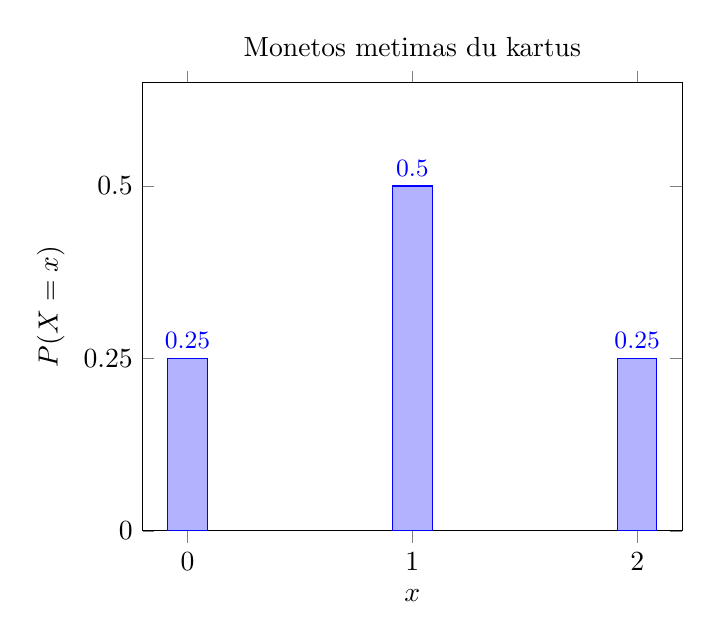
\begin{tikzpicture}
\begin{axis}[
  ybar, bar width=0.5cm,
  xlabel={$x$}, ylabel={$P(X=x)$},
  xtick={0,1,2},
  ytick={0, 0.25, 0.5},
  ymin=0, ymax=0.65,
  title={Monetos metimas du kartus},
  nodes near coords,
  every node near coord/.append style={font=\small},
]
\addplot coordinates {(0, 0.25) (1, 0.5) (2, 0.25)};
\end{axis}
\end{tikzpicture}
\end{center}

%---------------------------------------------------------
\subsection{Vidurkis ir dispersija}

\subsubsection*{Matematinė viltis (vidurkis)}

\begin{definition}
Diskrečiojo atsitiktinio dydžio $X$ \textbf{matematinė viltis} (arba \textbf{vidurkis}) $E(X)$ – tai svertinis reikšmių vidurkis, kur svoriai yra jų tikimybės:
\[
E(X) = x_1 p_1 + x_2 p_2 + \cdots + x_n p_n = \sum_{i=1}^{n} x_i p_i.
\]
\end{definition}

Matematinė viltis parodo, kokią reikšmę atsitiktinis dydis \emph{vidutiniškai} įgys atliekant daug bandymų. Ji yra \textbf{skirstinio centras svorių prasme}.

\begin{remark}
Matematinė viltis nebūtinai sutampa su nė viena iš galimų reikšmių. Pavyzdžiui, metant teisingą kauliuką, $E(X) = 3{,}5$, nors tokio taško nėra.
\end{remark}

\begin{example}
Remiantis ankstesniame skyrelyje sudarytu monetos skirstiniu:
\[
E(X) = 0 \cdot \frac{1}{4} + 1 \cdot \frac{1}{2} + 2 \cdot \frac{1}{4} = 0 + \frac{1}{2} + \frac{1}{2} = 1.
\]
Vidutiniškai tikimasi gauti 1 herbą per du metimus – tai intuityviai suprantama.
\end{example}

\subsubsection*{Matematinės vilties savybės}

\begin{theorem}[Matematinės vilties savybės]
Tegu $X$ – atsitiktinis dydis, $a, b \in \mathbb{R}$ – konstantos. Tada:
\begin{enumerate}
  \item $E(a) = a$,
  \item $E(aX) = a \cdot E(X)$,
  \item $E(X + a) = E(X) + a$,
  \item $E(aX + b) = a \cdot E(X) + b$.
\end{enumerate}
\end{theorem}

\subsubsection*{Binominio skirstinio vidurkis}

Jei $X \sim B(n, p)$ (binominis atsitiktinis dydis), tai:
\[
E(X) = np.
\]

\begin{example}
Šaulys šaudo 5 kartus, $p = 0{,}6$. Vidutinis pataikymų skaičius:
\[
E(X) = 5 \cdot 0{,}6 = 3.
\]
\end{example}

\subsubsection*{Dispersija}

\begin{definition}
\textbf{Dispersija} $D(X)$ – tai reikšmių nuokrypio nuo vidurkio kvadratų svertinis vidurkis:
\[
D(X) = \sum_{i=1}^{n} (x_i - E(X))^2 \, p_i.
\]
\end{definition}

Dispersija parodo, kaip plačiai atsitiktinio dydžio reikšmės \emph{išsibarsčiusios} aplink vidurkį. Kuo didesnė dispersija, tuo reikšmės labiau nutolę nuo vidurkio.

\begin{remark}
Praktikoje dažnai naudojama alternatyvi formulė, patogesnė skaičiavimams:
\[
D(X) = E(X^2) - \bigl[E(X)\bigr]^2,
\]
kur $E(X^2) = \displaystyle\sum_{i=1}^{n} x_i^2 \, p_i$.
\end{remark}

\begin{example}
Apskaičiuokime monetos metimo (du kartus) dispersiją. Žinome, kad $E(X) = 1$.

\begin{align*}
D(X) &= (0-1)^2 \cdot \frac{1}{4} + (1-1)^2 \cdot \frac{1}{2} + (2-1)^2 \cdot \frac{1}{4} \\
     &= 1 \cdot \frac{1}{4} + 0 + 1 \cdot \frac{1}{4} = \frac{1}{2}.
\end{align*}

Arba naudojant alternatyvią formulę:
\[
E(X^2) = 0^2 \cdot \frac{1}{4} + 1^2 \cdot \frac{1}{2} + 2^2 \cdot \frac{1}{4} = 0 + \frac{1}{2} + 1 = \frac{3}{2},
\]
\[
D(X) = \frac{3}{2} - 1^2 = \frac{1}{2}. \checkmark
\]
\end{example}

\subsubsection*{Standartinis nuokrypis}

\begin{definition}
\textbf{Standartinis nuokrypis} $\sigma(X)$ – tai dispersijos kvadratinė šaknis:
\[
\sigma(X) = \sqrt{D(X)}.
\]
Standartinis nuokrypis išreiškiamas tomis pačiomis matavimo vienetais kaip ir pats atsitiktinis dydis, todėl yra intuityvesnis išsibarstymo matas.
\end{definition}

\subsubsection*{Binominio skirstinio dispersija}

Jei $X \sim B(n, p)$, tada:
\[
D(X) = npq = np(1-p), \qquad \sigma(X) = \sqrt{np(1-p)}.
\]

\begin{example}
Tęsdami ankstesnį pavyzdį ($n = 5$, $p = 0{,}6$, $q = 0{,}4$):
\[
D(X) = 5 \cdot 0{,}6 \cdot 0{,}4 = 1{,}2, \qquad \sigma(X) = \sqrt{1{,}2} \approx 1{,}095.
\]
\end{example}

\subsubsection*{Palyginamoji lentelė}

\begin{center}
\begin{tabular}{|l|c|c|}
\hline
\textbf{Charakteristika} & \textbf{Formulė (bendrai)} & \textbf{Binominis $B(n,p)$} \\
\hline
Matematinė viltis & $\displaystyle\sum_{i} x_i p_i$ & $np$ \\
\hline
Dispersija & $\displaystyle\sum_{i}(x_i - E(X))^2 p_i$ & $npq$ \\
\hline
Standartinis nuokrypis & $\sqrt{D(X)}$ & $\sqrt{npq}$ \\
\hline
\end{tabular}
\end{center}

\begin{exercise}
Atsitiktinio dydžio $X$ skirstinys yra toks:
\[
\begin{array}{|c|c|c|c|}
\hline
X & -1 & 0 & 3 \\
\hline
P & 0{,}2 & 0{,}5 & 0{,}3 \\
\hline
\end{array}
\]
\begin{enumerate}[label=\alph*)]
  \item Apskaičiuokite $E(X)$.
  \item Apskaičiuokite $D(X)$ ir $\sigma(X)$.
  \item Raskite $E(2X + 1)$.
\end{enumerate}
\end{exercise}

\begin{exercise}
Teisingas kauliukas metamas 12 kartų. Tegu $X$ – šešetų skaičius.
\begin{enumerate}[label=\alph*)]
  \item Kokio tipo skirstinį turi $X$? Įvardykite parametrus.
  \item Apskaičiuokite $E(X)$, $D(X)$ ir $\sigma(X)$.
  \item Raskite tikimybę, kad šešetukas iškris lygiai 3 kartus.
\end{enumerate}
\end{exercise}

\section{Statistika}

Statistika – mokslas, tiriantis duomenų rinkimą, tvarkymą, analizę ir interpretavimą.
Ji padeda priimti pagrįstus sprendimus remiantis surinktais faktais. Šiame skyriuje
aptarsime pagrindines statistikos sąvokas ir rodiklius, reikalingus VBE egzaminui.

% ----------------------------------------------------------------
\subsection{Imtis ir statistiniai rodikliai}
% ----------------------------------------------------------------

\begin{definition}[Populiacija]
\textbf{Populiacija} (generalinė aibė) – visa tiriamų objektų (asmenų, daiktų,
reiškinių) aibė, apie kurią norima gauti informaciją.
\end{definition}

\begin{definition}[Imtis]
\textbf{Imtis} – iš populiacijos atsitiktinai atrinkta dalis objektų, kuri
naudojama populiacijos savybėms apibūdinti. Imties elementų skaičius žymimas $n$
ir vadinamas \textbf{imties dydžiu}.
\end{definition}

Statistinis tyrimas atliekamas šiais etapais:
\begin{enumerate}
  \item Tyrimo tikslo ir populiacijos nustatymas.
  \item Duomenų rinkimas (anketos, stebėjimas, eksperimentas).
  \item Duomenų tvarkymas ir sisteminimas.
  \item Statistinių rodiklių skaičiavimas.
  \item Išvadų formulavimas ir interpretavimas.
\end{enumerate}

\subsubsection*{Variacinė eilutė ir dažnių lentelė}

Surinkus duomenis, jie surašomi \textbf{variacine eilute} – reikšmės išdėstomos
didėjimo tvarka:
\[
  x_1 \leq x_2 \leq x_3 \leq \cdots \leq x_n.
\]

\begin{definition}[Dažnis]
\textbf{Dažnis} $m_k$ – skaičius, rodantis, kiek kartų konkreti reikšmė $x_k$
pasirodo imtyje. Visų dažnių suma lygi imties dydžiui:
\[
  m_1 + m_2 + \cdots + m_r = n.
\]
\end{definition}

\begin{definition}[Santykinis dažnis]
\textbf{Santykinis dažnis} $p_k$ – dažnio ir imties dydžio santykis:
\[
  p_k = \frac{m_k}{n}.
\]
Santykinis dažnis rodo, kokią dalį visos imties sudaro $k$-toji reikšmė.
Visų santykinių dažnių suma lygi 1:
\[
  p_1 + p_2 + \cdots + p_r = 1.
\]
\end{definition}

\begin{definition}[Procentinis dažnis]
\textbf{Procentinis dažnis} – santykinis dažnis, išreikštas procentais:
\[
  p_k^{\%} = \frac{m_k}{n} \cdot 100\%.
\]
\end{definition}

\subsubsection*{Pagrindiniai imties rodikliai}

\begin{definition}[Imties plotis]
\textbf{Imties plotis} $r$ – didžiausios ir mažiausios imties reikšmės skirtumas:
\[
  r = x_d - x_m,
\]
kur $x_d$ – didžiausia imties reikšmė, $x_m$ – mažiausia imties reikšmė.
\end{definition}

\begin{definition}[Imties centras]
\textbf{Imties centras} $c$ – didžiausios ir mažiausios reikšmės aritmetinis vidurkis:
\[
  c = \frac{x_d + x_m}{2}.
\]
\end{definition}

\subsubsection*{Duomenų vaizdavimas}

Statistiniai duomenys vaizduojami grafinėmis priemonėmis:
\begin{itemize}
  \item \textbf{Stulpelinė diagrama} – kiekvienas stulpelis atitinka tam tikrą
        reikšmę arba reikšmių grupę; stulpelio aukštis proporcingas dažniui.
  \item \textbf{Skritulinė diagrama} – ratas padalintas į sektorius; kiekvieno
        sektoriaus kampas proporcingas santykiniam dažniui ($360° \cdot p_k$).
  \item \textbf{Histograma} – naudojama sugrupuotiems (intervaliniams) duomenims;
        stulpeliai liečiasi vienas kito.
\end{itemize}

\begin{example}
Klasėje atliktas tyrimas ir gauti 10 mokinių matematikos įvertiniai:
\[
  7,\; 8,\; 6,\; 9,\; 7,\; 10,\; 8,\; 7,\; 6,\; 8.
\]
Variacinė eilutė: $6, 6, 7, 7, 7, 8, 8, 8, 9, 10$.

Sudarome dažnių lentelę:

\begin{center}
\begin{tabular}{|c|c|c|c|}
\hline
\textbf{Įvertinimas} $x_k$ & \textbf{Dažnis} $m_k$ & \textbf{Sant. dažnis} $p_k$ & \textbf{Proc. dažnis} \\
\hline
6  & 2 & 0,2 & 20\% \\
7  & 3 & 0,3 & 30\% \\
8  & 3 & 0,3 & 30\% \\
9  & 1 & 0,1 & 10\% \\
10 & 1 & 0,1 & 10\% \\
\hline
\textbf{Viso} & 10 & 1,0 & 100\% \\
\hline
\end{tabular}
\end{center}

Imties plotis: $r = 10 - 6 = 4$.

Imties centras: $c = \dfrac{10 + 6}{2} = 8$.
\end{example}

% ----------------------------------------------------------------
\subsection{Vidurkis, mediana, moda}
% ----------------------------------------------------------------

Centrinės tendencijos charakteristikos apibūdina imties „centrą" – tipinę ar
vidutinę reikšmę. Trys pagrindinės tokios charakteristikos yra \textbf{vidurkis},
\textbf{mediana} ir \textbf{moda}.

\subsubsection*{Imties vidurkis}

\begin{definition}[Aritmetinis vidurkis]
\textbf{Imties vidurkis} $\bar{x}$ – visų imties elementų reikšmių suma, padalinta
iš elementų skaičiaus:
\[
  \bar{x} = \frac{x_1 + x_2 + \cdots + x_n}{n} = \frac{1}{n}\sum_{i=1}^{n} x_i.
\]
\end{definition}

Kai duomenys pateikti dažnių lentele (sugrupuoti), vidurkis skaičiuojamas pagal formulę:

\begin{tcolorbox}[colback=blue!5!white, colframe=blue!60!black, title=Sugrupuotos imties vidurkis]
\[
  \bar{x} = \frac{x_1 m_1 + x_2 m_2 + \cdots + x_r m_r}{n}
            = \frac{\displaystyle\sum_{k=1}^{r} x_k m_k}{n},
\]
kur $x_k$ – $k$-toji reikšmė, $m_k$ – jos dažnis, $n$ – imties dydis.
\end{tcolorbox}

Arba naudojant santykinius dažnius:
\[
  \bar{x} = x_1 p_1 + x_2 p_2 + \cdots + x_r p_r = \sum_{k=1}^{r} x_k p_k.
\]

\begin{remark}
Vidurkis yra jautrus kraštinėms (labai didelėms arba labai mažoms) reikšmėms –
jos gali stipriai paveikti vidurkio reikšmę.
\end{remark}

\subsubsection*{Mediana}

\begin{definition}[Mediana]
\textbf{Mediana} $M_e$ – variacinės eilutės vidurinis elementas. Ji dalija
variacinę eilutę į dvi lygias dalis.
\begin{itemize}
  \item Jei imties dydis $n$ yra \textbf{nelyginis}: mediana yra
        $\left(\dfrac{n+1}{2}\right)$-asis elementas variacinėje eilutėje.
  \item Jei imties dydis $n$ yra \textbf{lyginis}: mediana yra dviejų vidurinių
        elementų aritmetinis vidurkis:
        \[
          M_e = \frac{x_{n/2} + x_{n/2+1}}{2}.
        \]
\end{itemize}
\end{definition}

\begin{remark}
Mediana atspari kraštinėms reikšmėms ir dažnai geriau nei vidurkis apibūdina
„tipinę" reikšmę, kai duomenys yra asimetriški (pvz., gyventojų pajamos).
\end{remark}

\subsubsection*{Moda}

\begin{definition}[Moda]
\textbf{Moda} $M_o$ – dažniausiai pasikartojanti imties reikšmė.
\begin{itemize}
  \item Moda gali būti \textbf{viena}, jei viena reikšmė pasikartoja dažniau nei
        visos kitos.
  \item Modos gali būti \textbf{kelios}, jei kelios reikšmės pasikartoja vienodai
        dažnai (ir tai yra didžiausias dažnis).
  \item Imtis \textbf{neturi modos}, jei visos reikšmės pasikartoja vienodą
        skaičių kartų.
\end{itemize}
\end{definition}

\begin{example}
Duota imtis: $3,\; 7,\; 7,\; 4,\; 5,\; 7,\; 3,\; 5,\; 8,\; 3,\; 7$.

Surašome variacine eilute: $3, 3, 3, 4, 5, 5, 7, 7, 7, 7, 8$. Čia $n = 11$.

\textbf{Vidurkis:}
\[
  \bar{x} = \frac{3+3+3+4+5+5+7+7+7+7+8}{11} = \frac{59}{11} \approx 5{,}36.
\]

\textbf{Mediana:} $n = 11$ – nelyginis, todėl mediana yra $\dfrac{11+1}{2} = 6$-asis
elementas variacinėje eilutėje: $M_e = 5$.

\textbf{Moda:} skaičius $7$ pasikartoja 4 kartus (daugiau nei visi kiti), todėl
$M_o = 7$.
\end{example}

\begin{example}
Duota imtis: $2,\; 4,\; 6,\; 8,\; 10,\; 12$.

Variacinė eilutė: $2, 4, 6, 8, 10, 12$. Čia $n = 6$ – lyginis.

\textbf{Mediana:}
\[
  M_e = \frac{x_3 + x_4}{2} = \frac{6 + 8}{2} = 7.
\]

\textbf{Moda:} kiekviena reikšmė pasikartoja po vieną kartą – imtis
\textbf{neturi modos}.
\end{example}

\subsubsection*{Centrinių charakteristikų palyginimas}

\begin{center}
\begin{tabular}{|l|p{4.5cm}|p{4.5cm}|}
\hline
\textbf{Rodiklis} & \textbf{Privalumai} & \textbf{Trūkumai} \\
\hline
Vidurkis $\bar{x}$ &
  Naudoja visas reikšmes; matematiškai patogus tolimesniems skaičiavimams &
  Jautrus išskirtims (ekstremalus reikšmėms) \\
\hline
Mediana $M_e$ &
  Atspari išskirtims; tinka asimetriniams duomenims &
  Neatsižvelgia į visų reikšmių dydį \\
\hline
Moda $M_o$ &
  Lengvai suprantama; tinka kokybiniams duomenims &
  Gali neegzistuoti arba būti neviena \\
\hline
\end{tabular}
\end{center}

% ----------------------------------------------------------------
\subsection{Standartinis nuokrypis}
% ----------------------------------------------------------------

Centrinės tendencijos rodikliai neapibūdina, kaip labai duomenys išsisklaidę apie
vidurkį. Šiam tikslui naudojami \textbf{sklaidos rodikliai}: dispersija ir
standartinis nuokrypis.

\subsubsection*{Dispersija}

\begin{definition}[Imties dispersija]
\textbf{Imties dispersija} $s^2$ – vidutinis kvadratinių nuokrypių nuo vidurkio
dydis. Skaičiuojama pagal formulę:
\[
  s^2 = \frac{(x_1 - \bar{x})^2 + (x_2 - \bar{x})^2 + \cdots + (x_n - \bar{x})^2}{n-1}
      = \frac{\displaystyle\sum_{i=1}^{n}(x_i - \bar{x})^2}{n-1}.
\]
\end{definition}

\begin{remark}
Vardiklyje rašoma $n-1$ (o ne $n$), nes imties dispersija turi būti \emph{neiškreiptas}
populiacijos dispersijos įvertinys. Kai $n$ didelis, skirtumas tarp $n$ ir $n-1$
yra nereikšmingas.
\end{remark}

Kai duomenys pateikti dažnių lentele:
\[
  s^2 = \frac{\displaystyle\sum_{k=1}^{r}(x_k - \bar{x})^2 \cdot m_k}{n-1}.
\]

Alternatyvi formulė su santykiniais dažniais (patogi skaičiavimams):
\[
  s^2 = \sum_{k=1}^{r} x_k^2 \cdot p_k - \bar{x}^2.
\]

\begin{remark}
Dispersija visada yra neneigiama: $s^2 \geq 0$. Dispersija lygi nuliui tik tada,
kai visos imties reikšmės yra vienodos.
\end{remark}

\subsubsection*{Standartinis nuokrypis}

\begin{definition}[Standartinis nuokrypis]
\textbf{Imties standartinis nuokrypis} $s$ – dispersijos kvadratinė šaknis:
\[
  s = \sqrt{s^2} = \sqrt{\frac{\displaystyle\sum_{i=1}^{n}(x_i - \bar{x})^2}{n-1}}.
\]
\end{definition}

\begin{tcolorbox}[colback=green!5!white, colframe=green!60!black,
  title=Standartinio nuokrypio savybės]
\begin{itemize}
  \item $s \geq 0$ visada.
  \item $s = 0$ tada ir tik tada, kai visos reikšmės lygios.
  \item $s$ matuojamas \textbf{tais pačiais vienetais} kaip ir imties duomenys,
        todėl jį lengva interpretuoti.
  \item Kuo didesnis $s$, tuo labiau duomenys išsisklaidę apie vidurkį.
  \item Jei kiekvienas imties elementas padidinamas $c$ kartų ($c > 0$), tai
        standartinis nuokrypis taip pat padidėja $c$ kartų.
  \item Jei kiekvienas imties elementas padidinamas (arba sumažinamas) tuo pačiu
        skaičiumi $a$, standartinis nuokrypis nesikeičia.
\end{itemize}
\end{tcolorbox}

\subsubsection*{Skaičiavimo algoritmas}

Standartiniam nuokrypiui apskaičiuoti rekomenduojama naudoti tokį algoritmą:

\begin{enumerate}
  \item Apskaičiuoti imties vidurkį $\bar{x}$.
  \item Kiekvienai reikšmei $x_i$ apskaičiuoti nuokrypį nuo vidurkio: $x_i - \bar{x}$.
  \item Kiekvieną nuokrypį pakelti kvadratu: $(x_i - \bar{x})^2$.
  \item Susumuoti visus kvadratinius nuokrypius: $\sum(x_i - \bar{x})^2$.
  \item Padalyti iš $n - 1$ – gauti dispersiją $s^2$.
  \item Ištraukti kvadratinę šaknį – gauti standartinį nuokrypį $s$.
\end{enumerate}

\begin{example}
Apskaičiuokite imties $\{2,\; 4,\; 4,\; 4,\; 5,\; 5,\; 7,\; 9\}$ standartinį nuokrypį.

\textbf{1 žingsnis. Vidurkis:}
\[
  \bar{x} = \frac{2+4+4+4+5+5+7+9}{8} = \frac{40}{8} = 5.
\]

\textbf{2–3 žingsniai. Nuokrypiai ir jų kvadratai:}

\begin{center}
\begin{tabular}{|c|c|c|}
\hline
$x_i$ & $x_i - \bar{x}$ & $(x_i - \bar{x})^2$ \\
\hline
2 & $-3$ & 9 \\
4 & $-1$ & 1 \\
4 & $-1$ & 1 \\
4 & $-1$ & 1 \\
5 & $0$  & 0 \\
5 & $0$  & 0 \\
7 & $2$  & 4 \\
9 & $4$  & 16 \\
\hline
  & \textbf{Suma} & 32 \\
\hline
\end{tabular}
\end{center}

\textbf{4–6 žingsniai. Dispersija ir standartinis nuokrypis:}
\[
  s^2 = \frac{32}{8 - 1} = \frac{32}{7} \approx 4{,}571,
\]
\[
  s = \sqrt{\frac{32}{7}} = \frac{4\sqrt{2}}{\sqrt{7}} \approx 2{,}138.
\]
\end{example}

\begin{example}
Duomenys pateikti dažnių lentele:

\begin{center}
\begin{tabular}{|c|c|c|}
\hline
$x_k$ & $m_k$ & $p_k$ \\
\hline
1 & 2 & 0,1 \\
3 & 4 & 0,2 \\
5 & 8 & 0,4 \\
7 & 4 & 0,2 \\
9 & 2 & 0,1 \\
\hline
\end{tabular}
\end{center}

$n = 20$. Naudojame santykinių dažnių formulę.

\textbf{Vidurkis:}
\[
  \bar{x} = 1\cdot0{,}1 + 3\cdot0{,}2 + 5\cdot0{,}4 + 7\cdot0{,}2 + 9\cdot0{,}1
          = 0{,}1 + 0{,}6 + 2{,}0 + 1{,}4 + 0{,}9 = 5.
\]

\textbf{Dispersija} (alternatyvia formule):
\[
  s^2 = \sum x_k^2 p_k - \bar{x}^2
      = (1\cdot0{,}1 + 9\cdot0{,}2 + 25\cdot0{,}4 + 49\cdot0{,}2 + 81\cdot0{,}1) - 25
\]
\[
      = (0{,}1 + 1{,}8 + 10{,}0 + 9{,}8 + 8{,}1) - 25
      = 29{,}8 - 25 = 4{,}8.
\]

\textbf{Standartinis nuokrypis:}
\[
  s = \sqrt{4{,}8} \approx 2{,}19.
\]
\end{example}

\subsubsection*{Standartinio nuokrypio interpretacija}

\begin{tcolorbox}[colback=yellow!5!white, colframe=orange!80!black,
  title=Praktinė interpretacija]
Tarkime, mokinių ūgių imties vidurkis $\bar{x} = 170$ cm ir standartinis nuokrypis
$s = 5$ cm. Tai reiškia, kad daugelio mokinių ūgis nukrypsta nuo vidurkio maždaug
5 cm, t.~y. daugelio mokinių ūgis yra intervale $[165,\; 175]$ cm.

Jei kitos imties standartinis nuokrypis $s' = 12$ cm, tai tos imties duomenys yra
labiau išsibarstę.
\end{tcolorbox}

\subsubsection*{Pagrindinių rodiklių santrauka}

\begin{center}
\begin{tabular}{|l|l|}
\hline
\textbf{Rodiklis} & \textbf{Formulė} \\
\hline
Imties plotis & $r = x_d - x_m$ \\
Imties centras & $c = \dfrac{x_d + x_m}{2}$ \\
Santykinis dažnis & $p_k = \dfrac{m_k}{n}$ \\
Vidurkis & $\bar{x} = \dfrac{\sum x_i}{n}$ \\
Sugrupuotos imties vidurkis & $\bar{x} = \dfrac{\sum x_k m_k}{n}$ \\
Dispersija & $s^2 = \dfrac{\sum(x_i-\bar{x})^2}{n-1}$ \\
Standartinis nuokrypis & $s = \sqrt{s^2}$ \\
\hline
\end{tabular}
\end{center}

\begin{exercise}
Dešimties šuolių į aukštį rezultatai (cm):
\[
  155,\; 160,\; 158,\; 162,\; 157,\; 165,\; 159,\; 161,\; 163,\; 160.
\]
\begin{enumerate}[label=\alph*)]
  \item Surašykite variacine eilute ir sudarykite dažnių lentelę.
  \item Apskaičiuokite imties plotį ir centrą.
  \item Raskite vidurkį, medianą ir modą.
  \item Apskaičiuokite dispersiją ir standartinį nuokrypį.
\end{enumerate}
\end{exercise}

\begin{exercise}
Duomenys pateikti dažnių lentele:
\begin{center}
\begin{tabular}{|c|c|c|c|c|c|}
\hline
$x_k$ & 10 & 20 & 30 & 40 & 50 \\
\hline
$m_k$ & 3  & 7  & 15 & 7  & 3  \\
\hline
\end{tabular}
\end{center}
Raskite vidurkį ir standartinį nuokrypį.
\end{exercise}

